%************************************************
\chapter{Calibración de la cámara}\label{ch:calibracion}
%************************************************

Este capítulo se dedica exclusivamente a la calibración de la cámara. Este es uno de los aspectos más importantes del proyecto, considerando que la cámara es el principal elemento que utilizaremos para realizar mediciones.

En la primer sección se realiza una introducción para entender mejor a qué nos referimos cuando hablamos de la calibración de la cámara. 
En la segunda sección se explicarán de manera sencilla algunos conceptos de la óptica relacionados con el funcionamiento de una cámara fotográfica.
En la tercer sección se explica el funcionamiento de una cámara de fotos digital y la manera en la que se obtienen las imágenes.
En la cuarta sección se introduce un modelo de cámara simple conocido como \emph{cámara pinhole}.
En la quinta sección se extiende el modelo de cámara pinhole para incluir las distorsiones ópticas más frecuentes.
En la sexta sección se explica el concepto de parámetros extrínsecos de una cámara.
La séptima sección puede considerarse la más importante, en la cual se explica un método para obtener los párametros del modelo de cámara, incluyendo los parámetros extrínsecos y los que modelan la distorsión.
Finalmente en la última sección se trata brevemente la calibración conjunta de más de una cámara.

\section{Introducción}\label{sec:calibracion_intro}
Una cámara fotográfica realiza un mapeo desde el mundo en tres dimensiones (3D) hacia una imagen (dos dimensiones, 2D). A lo largo de los años diversos modelos matemáticos han sido propuestos para describir este mapeo. En palabras simples, un modelo matemático de una cámara describe cómo se proyectan los objetos en tres dimensiones sobre la imagen y viceversa, cómo proyectar desde la imagen hacia el espacio tridimensional. La calibración de una cámara consiste en determinar los parámetros de este modelo. Este problema incluye el modelado y la parametrización del proceso completo de obtención de las imágenes.

Los modelos de cámaras pueden ser clasificados de acuerdo a diferentes criterios, como por ejemplo en el uso de la suposición (o no) de que existe un único punto por el que pasan todos los rayos de luz. Los modelos que utilizan esta suposición son conocidos como modelos de cámara centrales, y el resto como no centrales. Otra clasificación puede hacerse entre modelos globales, locales o discretos. En los modelos globales el cambio de un parámetro afecta a todo el campo de visión, en cambio en los modelos locales el cambio de un parámetro afecta sólo a una zona. Por otro lado un modelo discreto es aquel que tiene un grupo de parámetros para cada punto de la imagen \cite{sturm2011camera}.

En este trabajo vamos a utilizar un modelo de cámara central y global, conocido generalmente como modelo de cámara pinhole. El uso de un modelo de cámara central nos permite formular el mapeo como una proyección. Esto nos posibilita utilizar todos los conceptos de la geometría proyectiva \cite{hanning2011high}.

Muchas aplicaciones de visión por computadora no requieren alta precisión en la reconstrucción. Por ejemplo en robótica muchas veces solamente es necesario obtener información sobre un entorno desconocido. En estos casos puede ser más importante estimar la orientación del sensor que medir distancias con exactitud. En otros casos donde se busca reconstruir dimensiones con exactitud -como el planteado en este trabajo-, el modelo de la cámara pinhole debe ser extendido con un modelo de distorsión que generalmente se define en el plano de la imagen. Este modelo, aún siendo sólo una aproximación del comportamiento real de la cámara, nos permitirá incrementar considerablemente la calidad de nuestros resultados.

\section{Sistema óptico de la cámara}
Las cámaras funcionan detectando rayos de luz. Los rayos provenientes de alguna fuente de luz viajan por el espacio hasta los objetos. El objeto absorbe parte de esa luz y el resto es reflejado. Parte de estos rayos pueden ser reflejados hacia la cámara, donde se produce una imagen. Para poder obtener información del mundo real a partir de la imagen necesitamos conocer en detalle lo que sucede con el rayo de luz al pasar por la lente y en qué lugar es capturado por el sensor de la cámara.

En nuestro caso vamos a analizar el sistema óptico con la ayuda de la óptica geométrica. Se define la óptica geométrica como aquella que abarca el estudio de los fenómenos relativos a la propagación de la luz sin incluir los efectos de interferencia ni de difracción, considerando los objetos compuestos por un conjunto de fuentes radiantes puntuales independientes. Esta descripción, basada en el análisis de las trayectorias (rayos) de propagación de la energía, es válida siempre que la longitud de onda de la perturbación que se desplaza sea mucho menor que las dimensiones características de los objetos con los que se encuentra \cite{greivenkamp2004field}.

También asumiremos que la lente es simétrica alrededor de un eje de rotación que denominaremos eje óptico de la lente.

\subsection{Óptica de primer orden}
La óptica geométrica se basa en la ley de refracción, también conocida como ley de Snell. Dados dos medios con índices de refracción $n_1$ y $n_2$ y un rayo de luz que pasa desde el medio $1$ al medio $2$, como se observa en la \autoref{fig:snellsLaw}, la ley de refracción establece que los ángulos $\theta_1$ y $\theta_2$ del rayo respecto a la normal de la interfaz entre los medios es:
\begin{equation*}
	n_1 \sin(\theta_1) = n_2 \sin(\theta_2)
\end{equation*}
\begin{figure}[bth]
    \centering
        {\includegraphics[width=.6\linewidth]{images/snellsLaw}}
        \caption{Rayo de luz atravesando un medio}
        \label{fig:snellsLaw}
\end{figure}

En el ámbito de la visión por computadora generalmente se acepta que el índice de refracción del aire es tan cercano a 1 que se trata como si fuera igual a 1 \cite{hanning2011high}. Una lente esférica tiene dos interfaces entre medios (aire-lente y lente-aire) los cuales se describen como dos esferas con el mismo radio $r$, como se observa en la \autoref{fig:sphericalLens}.
\begin{figure}[bth]
    \centering
        {\includegraphics[width=.5\linewidth]{images/sphericalLens}}
        \caption{Lente esférica}
        \label{fig:sphericalLens}
\end{figure}

Mediante la ley de Snell podemos reconstruir la refracción de cada rayo proveniente de un objeto que pasa por la lente.

En óptica de primer orden se asume que todos los rayos de luz considerados en el modelo de la cámara son casi paralelos al eje óptico de la lente. En este caso todos los ángulos respecto a la normal de la superficie de la lente son pequeños, por lo que podemos aproximar el seno como $\sin(x) \approx x$. Debido a que esta aproximación es el primer término de la aproximación de Taylor para el seno, las derivaciones que siguen esta suposición son conocidas como \emph{óptica de primer orden}.

Otra suposición que se realiza comúnmente en visión por computadora es llamada suposición de lente delgada: se asume que la lente es infinitesimalmente fina. Desde el punto de vista de la refracción una lente delgada se comporta como una lente esférica, pero la distancia recorrida por el rayo en el interior de la lente es infinitesimalmente pequeña. Por lo tanto podemos asumir que la lente es un plano. Este plano es generalmente llamado \emph{plano principal}. Un rayo de luz pasando por una lente de estas características es afectado por la ley de Snell en la interfaz aire-lente e inmediatamente afectado por la ley de Snell en la interfaz lente-aire. Una consecuencia de ésto es que cualquier rayo de luz que pase por el eje óptico de la lente no será afectado por la refracción, debido a que la superficie de ambas interfaces en este punto es paralela y la distancia entre ellas es nula. Otra consecuencia de este modelo de lente combinado con la simplificación de que todos los rayos son casi paralelos es que todos los rayos emitidos en un punto $p$ en un lado de la lente, al pasar por la lente se vuelven a encontrar en un punto $p_i$ al otro lado de la lente de manera que:
\begin{equation*}
    \frac{1}{d_p} + \frac{1}{d_i} = \frac{1}{f}
\end{equation*}
donde
\begin{equation*}
    f = \frac{r}{2(n_l-1)}        %--->esto no tiene mucho sentido, no era nl ~= 1? para el vidrio cuanto es?
\end{equation*} 
siendo $n_l$ el índice de refracción de la lente, y $d_p$ y $d_i$ la distancia del punto $p$ y $p_i$ al plano principal. Esto significa que hay una relación entre los objetos y la imagen, y que esta relación depende solamente de la distancia entre el objeto y el plano principal, y que no depende de la distancia hacia el eje óptico. Esta ecuación es conocida como \emph{ecuación del fabricante de lentes} (lens' maker equation).

Existe una distancia detrás del plano principal ($d_i$ en la \autoref{fig:lensFocalPlane}) para la cual la observación de un punto $p$ se transforma en una imagen enfocada. Se puede decir que cada plano paralelo al plano principal determina un plano focal detrás de la lente donde los puntos se ven enfocados.
\begin{figure}[bth]
    \centering
        {\includegraphics[width=1.\linewidth]{images/lensFocalPlane}}
        \caption{Rayo de luz atravesando un medio}
        \label{fig:lensFocalPlane}
\end{figure}

En la \autoref{fig:lensFocalPlane} se pueden observar tres rayos de luz que pasan por el modelo de lente delgada:
\begin{itemize}
\item El rayo que proviene de un lado en dirección paralela al eje óptico de la lente pasa por un punto $F$ al otro lado de la lente, ubicado a una distancia $f$ del plano principal. $F$ es denominado punto focal. La distancia $f$ es llamada \emph{distancia focal posterior}.
\item Un rayo que pasa por el centro de la lente no cambia su dirección. Este rayo es denominado rayo central. El centro de la lente es llamado \emph{centro óptico de la lente}.
\item Un rayo que arriba a la lente desde el punto $F'$ (ubicado a una distancia $f'$ del plano principal) sale de manera paralela al eje óptico del otro lado. La distancia de $F'$ al plano principal es llamada \emph{distancia focal anterior}.
\end{itemize}

A lo largo de este trabajo consideraremos una lente esférica con óptica de primer orden y con distancia focal posterior igual a la distancia focal anterior. Para una lente delgada con óptica de primer orden la distancia focal es independiente de la distancia del punto/objeto al eje óptico.

\subsection{El círculo de confusión}
Generalmente la adquisición de la imagen se produce mediante un sensor plano. Llamaremos a este plano donde se obtiene la imagen \emph{plano imagen}. Generalmente el plano imagen no coincide con el plano focal, por lo tanto no todos los rayos provenientes de los objetos en observación se cruzan en un punto sobre el plano imagen.

Si consideramos una fuente de luz puntual en el lado del objeto, todos los rayos provenientes de este punto que pasan la lente forman un cono en el otro lado de la lente. La intersección de este cono con el plano imagen se denomina \emph{círculo de confusión}.

Si el círculo de confusión es más pequeño que el tamaño de un elemento del sensor, el objeto aparecerá nítido, bien definido. El rango de posiciones del objeto (distancias a la cámara en dirección del eje focal) en el cual esto es cierto se denomina \emph{profundidad de campo} (depth of field).

Esta dependencia entre nitidez y profundidad puede ser usada para estimar la distancia a un objeto (la distancia del objeto al plano principal), y es utilizada por las técnicas denominadas \emph{depth from focus} ó \emph{depth from de-focus}.

Este efecto borroso de la óptica de primer orden también puede ser tenido en cuenta en el modelado de la cámara. La manera más común de manejar este efecto es mediante la convolución de la \emph{imagen ideal} con un kernel. La \emph{imagen ideal} es la imagen obtenida a partir de los rayos centrales únicamente, lo cual en la vida real es impracticable. En visión por computadora este kernel es también conocido como \ac{PSF}. El \ac{PSF} puede ser visto como la respuesta al impulso del sistema óptico. Existen diferentes maneras de estimar el \ac{PSF}, aunque en este trabajo no lo tendremos en cuenta.

\subsection{Óptica de tercer orden}
Como se dijo previamente, la simplificación $\sin(x) \approx x$ solamente es válida para ángulos pequeños. Un modelo de refracción más realista se obtiene truncando la serie de Taylor del seno en el término de tercer orden: $\sin(x) \approx x - \frac{1}{3!} x^3$. Esto nos lleva a la denominada óptica de tercer orden. Se puede comprobar fácilmente que en óptica de tercer orden la refracción de un rayo de luz si depende de la distancia al eje óptico.

También podemos expandir el modelo de lente al denominado modelo de lente gruesa, que puede ser modelado como dos lentes delgadas paralelas. Este modelo sumado a la óptica de tercer orden permiten modelar las aberraciones monocromáticas de un sistema óptico. A continuación describiremos rápidamente las denominadas cinco aberraciones de Seidel, las cuales pueden ser modeladas bajo las suposiciones de este modelo \cite{hanning2011high}.

\subsubsection{Aberraciones esféricas}
Rayos que inciden sobre la superficie de un lente esférico a mayor distancia del eje óptico enfocarán más cerca que rayos a menor distancia. Esto lleva a la aparición de un círculo de confusión incluso en el plano focal. Esta aberración puede ser eliminada usando una lente oval en vez de una esférica, pero estas lentes tienen un costo más elevado. Se puede observar un ejemplo de esta aberración en la \autoref{fig:aberration_spherical_coma}.
%\begin{figure}[bth]
%    \myfloatalign
%        {\includegraphics[width=0.6\linewidth]{images/aberration_spherical}}
%        \caption{Aberración esférica}
%        \label{fig:aberration_spherical}
%\end{figure}

\begin{figure}[bth]
    \myfloatalign
        \myfloatalign
        \subfloat[Aberración esférica]
        {\includegraphics[width=.40\linewidth]{images/aberration_spherical}} 
        \subfloat[Coma]
        {\includegraphics[width=.59\linewidth]{images/aberration_coma}}
        \caption{Aberraciones}\label{fig:aberration_spherical_coma}
\end{figure}

\subsubsection{Coma}
Rayos provenientes de un objeto que no está en el eje óptico serán enfocados en diferentes puntos. En sistemas no óptimos el enfoque puede ser asimétrico. La imagen de un punto aparece como gota en vez de como un círculo. Esta aberración afecta en mayor medida a los telescopios pero igualmente debemos tener en cuenta que transforma el círculo de confusión en una figura asimétrica. Se puede observar un ejemplo de esta aberración en la \autoref{fig:aberration_spherical_coma}.
%\begin{figure}[bth]
%    \myfloatalign
%        {\includegraphics[width=0.8\linewidth]{images/aberration_coma}}
%        \caption{Coma}
%        \label{fig:aberration_coma}
%\end{figure}

\subsubsection{Astigmatismo}
Rayos provenientes de un objeto alejado del eje óptico no incidirán de manera simétrica sobre la superficie de la lente. Esto hace que los rayos no enfoquen en un mismo punto, provocando una deformación elíptica del círculo de confusión. Se puede observar un ejemplo de esta aberración en la \autoref{fig:aberration_astigmatism}.
\begin{figure}[bth]
    \myfloatalign
        {\includegraphics[width=1.0\linewidth]{images/aberration_astigmatism}}
        \caption{Astigmatismo}
        \label{fig:aberration_astigmatism}
\end{figure}

\subsubsection{Curvatura de campo}
El comportamiento de la refracción en la óptica de tercer orden también impacta la relación entre objetos y puntos en la imagen. Para un plano objeto paralelo al plano principal de la lente, el área donde los puntos estarán enfocados no será un plano sino una superficie curva\footnote{Esta aberración también es conocida como \emph{Petzval field curvature}, en honor a Josef Petzval, que fue el primero en analizar este efecto}. Sólo se puede aproximar con un plano para puntos cercanos al eje óptico. Esto significa que no es teóricamente posible que todos los pixels de una imagen estén en foco si usamos una cámara con un array plano de sensores. Este efecto sin embargo no es significativo debido a que el tamaño del sensor es usualmente muy pequeño en comparación al objeto, aunque puede ocurrir por ejemplo en las fotografías en modo \emph{macro}. Se puede observar un ejemplo de esta aberración en la \autoref{fig:aberration_fieldCurvature}.
\begin{figure}[bth]
    \myfloatalign
        {\includegraphics[width=0.8\linewidth]{images/aberration_fieldCurvature}}
        \caption{Curvatura de campo}
        \label{fig:aberration_fieldCurvature}
\end{figure}

\subsubsection{Distorsión}
En óptica de tercer orden la magnificación transversal en el plano de la imagen se transforma en una función de la distancia al eje óptico, es decir radial. A diferencia de las aberraciones anteriores, la distorsión también afecta los rayos centrales. La distorsión (como la describe Seidel) está determinada completamente en el plano de la imagen.
%, por lo tanto puede ser modelada como una función en el plano ${z=1}$. 
Se puede observar ejemplos de este tipo de aberración en la \autoref{fig:aberration_distortion}.
\begin{figure}[bth]
    \myfloatalign
        \myfloatalign
        \subfloat[Barrel]
        {\includegraphics[width=.35\linewidth]{images/aberration_distortion_barrel}} 
        \quad \quad \quad
        \subfloat[Pincushion]
        {\includegraphics[width=.35\linewidth]{images/aberration_distortion_pincushion}}
        \caption[Distorsión]{Ejemplos de distorsión}\label{fig:aberration_distortion}
\end{figure}

\section{Adquisición de imágenes}
El sensor de la cámara es un dispositivo electrónico que convierte la intensidad de los rayos de luz en una señal eléctrica. Generalmente se trata de una grilla rectangular de elementos sensibles a la luz, y los más usados son del tipo \ac{CCD} ó \ac{CMOS}. Un esquema de la estructura de un sensor puede observarse en la \autoref{fig:cameraSensorArray}. Esta grilla rectangular establece el sistema de coordenadas canónico para la imagen.
\begin{figure}[bth]
    \myfloatalign
        {\includegraphics[width=0.8\linewidth]{images/cameraSensorArray}}
        \caption{Esquema del sensor de una cámara}
        \label{fig:cameraSensorArray}
\end{figure}

Cada sensor de la grilla determina el valor correspondiente a un elemento de la imagen (pixel), es decir que cada pixel representa un área rectangular del plano de la imagen.

El modelo simplificado del sensor de la cámara no considera:
\begin{itemize}
    \item la superficie no foto-sensitiva presente entre cada elemento foto-sensitivo del array
    \item la interacción entre los elementos foto sensitivos y sus vecinos, por ejemplo el ruido causado durante la lectura de los valores de cada elemento en cámaras de bajo costo,
    \item las diferencias entre los elementos foto-sensitivos. Se asume que todos tienen el mismo tamaño y las mismas características     
\end{itemize}

\section{Modelo de cámara pinhole}
Generalmente denominamos lente a lo que en realidad es un sistema de lentes, pero a fines prácticos lo que nos interesa es que las propiedades ópticas del sistema de lentes se aproximan a las propiedades ópticas de una lente delgada \emph{virtual}. El modelo pinhole se basa en el rayo central del modelo de lente delgada. El rayo central pasa por el centro de la lente para cada posición del objeto. Esto significa que podemos modelar la cámara como una \emph{cámara oscura}, con el centro óptico del lente como el \emph{pinhole}, como se observa en la \autoref{fig:pinholeCameraSchema}.
\begin{figure}[bth]
    \myfloatalign
        {\includegraphics[width=1.0\linewidth]{images/pinholeCameraSchema}}
        \caption{Modelo de cámara pinhole}
        \label{fig:pinholeCameraSchema}
\end{figure}

Para explicar el modelo de cámara pinhole vamos a definir dos sistemas de coordenadas: el sistema de coordenadas de la cámara (CCS) y el sistema de coordenadas de la imagen (ICS). El sistema de coordenadas de la cámara es un sistema de coordenadas cartesiano definido por el plano principal: los ejes $x$ e $y$ del CCS determinan el plano principal mientras que el eje $z$ viene dado por el eje óptico. El centro óptico del lente determina el origen $(0,0,0)$ del CCS. El plano principal queda definido entonces por ${z=0}$. 

El sistema de coordenadas de la imagen es el sistema de coordenadas canónico del array de sensores de la cámara. En nuestro caso vamos a asumir que el primer eje del sistema de coordenadas de la cámara es paralelo al primer eje del sistema de coordenadas de la imagen. La intersección del plano imagen con el eje óptico se denomina punto principal.

En este momento vamos a modificar el modelo pinhole a una forma equivalente pero que nos va a facilitar la comprensión: vamos a pensar que el plano de la imagen está delante del plano principal, como se muestra en la \autoref{fig:cameraProjectionModel}, es decir consideraremos que la imagen se forma en un plano virtual delante del centro óptico. El centro óptico se puede ver entonces como un centro de proyección.
\begin{figure}[bth]
    \myfloatalign
        {\includegraphics[width=1.0\linewidth]{images/cameraProjectionModel}}
        \caption{Modelo de proyección de la cámara}
        \label{fig:cameraProjectionModel}
\end{figure}

El hecho de que en el modelo pinhole todos los rayos desde el objeto hacia la imagen se intersectan en un punto (el centro óptico) nos permite utilizar una transformación proyectiva: la relación que asigna un punto $Q$ en el mundo físico con coordenadas $(X, Y, Z)$ a un punto $q$ del plano de proyección con coordenadas $(x, y)$ se llama transformación proyectiva. Cuando se trabaja con transformaciones de este tipo es conveniente usar lo que se conoce como coordenadas homogéneas. La coordenada homogénea asociada a un punto en un espacio proyectivo de dimensión $n$ se expresa típicamente como un vector de dimensión $n+1$, con la restricción adicional de que dos puntos cualesquiera cuyos valores son proporcionales serán equivalentes. En nuestro caso, el espacio proyectivo es el plano de la imagen, que posee dos dimensiones, por lo que vamos a representar los puntos que en él se encuentran como tridimensionales: $q = (x, y, w)$. Es posible recuperar las coordenadas en el plano de la imagen dividiendo las dos primeras componentes del vector por la tercera. De esta manera, se podrá disponer de los parámetros de la proyección en un matriz $M$ de $3x3$, que será denominada matriz intrínseca.
\begin{equation*}
    M =
    \begin{bmatrix}
        fx &  s & cx \\
         0 & fy & cy \\
         0 &  0 &  1
    \end{bmatrix}
\end{equation*}
donde $fx$ y $fy$ se pueden interpretar como la escala para los ejes $x$ e $y$ respectivamente, $cx$ y $cy$ es el punto principal respecto al ICS, y $s$ describe el skewness en el sistema de coordenadas de la imagen. Si $s$ es cero, los ejes $x$ e $y$ del sistema de coordenadas de la imagen son perpendiculares.

Como consideramos que el lente era simétrico alrededor del eje de proyección podríamos llegar a creer que $fx = fy$, sin embargo no siempre podemos usar esta simplificación ya que el array de sensores de la cámara puede tener diferente espaciado en cada dirección, o bien el elemento foto sensible puede ser rectangular en vez de cuadrado. Es por esto que lo dejaremos modelado por separado.

La proyección de los puntos del mundo físico (en coordenadas del CCS) hacia la cámara (en coordenadas del ICS) puede ahora escribirse en forma matricial:
\begin{equation*}
	[u, v, 1]^T = M [X, Y, Z]^T
\end{equation*}	
donde $u = x/z$ y $v = y/z$ son las coordenadas para los ejes $x$ e $y$ en el ICS.

\section{Modelo pinhole con distorsión}

Como se dijo previamente, la única aberración que afecta los rayos centrales es la distorsión. Por lo tanto, para el modelo de cámara pinhole, con solo considerar los efectos de la distorsión podemos lograr una aproximación a una óptica de tercer orden. Con este fin se introduce un modelo para corregir la distorsión en el plano de la imagen ${z=1}$. Este modelo es una función de dos variables, $x$ e $y$.

\subsection{Distorsión radial}

La mayoría de los lentes utilizados comúnmente son invariantes a la rotación. Se puede decir que existe un eje de rotación de la lente, y vamos a aceptar la suposición de que éste eje de rotación corresponde al eje óptico de nuestro modelo de cámara. De esta forma podemos ver que la distorsión producida por la lente depende únicamente de la distancia al eje óptico, el radio $r$.

Para cada punto $q = (x,y)$ perteneciente a $\mathbb{R}^2$ se define su dirección $n_q$ como
\begin{equation*}
    n_q = \frac{q}{||q||}
\end{equation*}
Una función de distorsión radial $c$ es una función que mapea:
\begin{equation*}
	q = ||q|| n_q   \mapsto   c(||q||) n_q
\end{equation*}
Esta función depende únicamente de la distancia de $q$ al origen, es decir, del radio $r = ||q||$. Se puede modelar la distorsión con cualquier función análitica, pero por comodidad la vamos a formular como una serie de Taylor:
\begin{equation*}
	c(||q||) = c(r) = \sum_{i=0}^{\infty} c_i r^i
\end{equation*}
Como asumimos que la distorsión es nula en el origen, fijamos el coeficiente constante $c_0 = 0$. A su vez fijamos el coeficiente lineal $c_1 = 1$, ya que es simplemente una escala alrededor del origen, y no puede ser $0$ ya que estaríamos excluyendo la distorsión nula como posible solución.
Nuestra función de distorsión queda entonces definida como:
\begin{equation*}
	c(r) = r + \sum_{i=2}^{\infty} c_i r^i = r (1 + \sum_{i=1}^{\infty} c_{i+1} r^i)
\end{equation*}
De esta forma:
\begin{equation*}
    \begin{aligned}
	q_{corregido} = c(||q||) n_q &= ||q|| (1 + \sum_{i=1}^{\infty} c_{i+1} ||q||^i) n_q\\
                                                         &= (1 + \sum_{i=1}^{\infty} c_{i+1} ||q||^i) q \\
                                                         &= q + q \sum_{i=1}^{\infty} c_{i+1} ||q||^i \\
    \end{aligned}
\end{equation*}	

Finalmente, como el radio sólo puede ser positivo, podemos asumir que $c$ puede ser aproximada por una función impar, lo que nos brinda la ventaja de que sólo debemos considerar los exponentes pares de la serie de potencias. Esta ventaja se hace evidente cuando debemos calcular el radio, ya que podemos obviar el cálculo de la raíz cuadrada para obtener $r = ||q||$.
De esta forma podemos escribir:
\begin{equation*}
	\begin{bmatrix}
	    x_{corregido} \\
	    y_{corregido} \\
	\end{bmatrix}
	= 
	\begin{bmatrix}
	    x (1 + k_1 r^2 + k_2 r^4 + k_3 r^6 + \dots + k_i r^{2i}) \\
	    y (1 + k_1 r^2 + k_2 r^4 + k_3 r^6 + \dots + k_i r^{2i}) \\
	\end{bmatrix}
\end{equation*}
con los $k_i$ como parámetros de distorsión radial.

\subsection{Distorsión tangencial}

La alineación de la lente en un sistema óptico también puede producir distorsiones. Estas distorsiones no pueden ser descritas como funciones que dependan solamente de la distancia al eje óptico.

En nuestro modelo de cámara asumimos que el plano de la imagen y el plano definido por el array de sensores eran paralelos. Por lo tanto cualquier desalineación entre ellos también debe ser modelado por la función de distorsión. Por ejemplo para lentes que están inclinados respecto al plano de la imagen (ver \autoref{fig:tangentialDistortionPossibleCause}) la distorsión radial se transforma en una distorsión elíptica.
\begin{figure}[bth]
    \myfloatalign
        {\includegraphics[width=1.0\linewidth]{images/tangentialDistortionPossibleCause}}
        \caption{Posible causante de distorsión tangencial}
        \label{fig:tangentialDistortionPossibleCause}
\end{figure}

Por otro lado, como se mencionó previamente, los sistemas de lentes reales generalmente son una combinación de dos o más lentes. Idealmente todas las lentes compartirán el mismo eje óptico. Sin embargo durante la construcción del sistema de lentes se pueden producir pequeñas diferencias, lo que también puede generar una aberración en la imagen observada.

Una característica de este tipo de aberraciones es que el eje óptico puede no ser el centro de la distorsión radial. Para modelar este tipo de casos se puede introducir una distorsión tangencial definida como \cite{bradski2008learning}:
\begin{equation*}
	\begin{bmatrix}
	    x_{corregido} \\
	    y_{corregido} \\
	\end{bmatrix}
	= 
	\begin{bmatrix}
	    x + [ 2 p_1 y + p_2 (r^2 + 2 x^2) ] \\
	    y + [ p_1 (r^2 + 2 y^2) + 2 p_2 x ] \\
	\end{bmatrix}
\end{equation*}
con $p_1$ y $p_2$ como parámetros de distorsión tangencial.

% este sale de Hanning pero no lo uso asi que mejor no ponerlo
%\begin{equation*}
%	\delta_{\text{tan}}(u,v) = 
%	\begin{bmatrix}
%	    t_1 (3 u^2 + v^2) + 2 t_2 u v \\
%	    t_2 (u^2 + 3 v^2) + 2 t_1 u v \\
%	\end{bmatrix}
%\end{equation*}
%con $t_1$ y $t_2$ como parámetros de distorsión.

Se pueden seguir añadiendo muchos otros modelos de distorsión, pero para nuestros fines la distorsión radial y tangencial resultan suficientes. Por otro lado se debe ser cuidadoso de que los parámetros que definen la distorsión completa sean independientes entre sí.

Como se comentó previamente, la transición de un sistema de coordenadas euclidiano a un sistema de coordenadas proyectivo nos permite utilizar matrices para realizar los cambios de sistemas de coordenadas. En este momento es importante destacar que, si bien el modelo de cámara que utilizamos (excepto la distorsión) consiste simplemente en una transformación del sistema de coordenadas, el modelo de distorsión debe ser tratado de manera separada ya que no se puede describir como una matriz. Debemos recordar que el modelo de distorsión que se presentó está definido y sólo actúa sobre el plano $z=1$ del sistema de coordenadas de la cámara.

\section{Parámetros extrínsecos}

Previamente cuando se introdujeron los parámetros intrínsecos de la cámara se asumió el hecho de que el centro óptico era el origen del sistema de coordenadas global. Sin embargo en diversas aplicaciones -como se verá más adelante en este proyecto- es necesario conocer la ubicación espacial de la cámara respecto a otro sistema de coordenadas. 

Para poder modelar el sistema con independencia de su posición o para poder referenciar un objeto respecto a otro origen de coordenadas es necesario introducir un cambio de coordenadas. Este cambio de coordenadas equivale a una transformación rígida compuesta de una rotación $R$ y una traslación $t$, como se observa en la \autoref{fig:rotationAndTraslation}. Gracias a que estamos trabajando con coordenadas homogéneas, podemos combinarlas en una sola matriz de $3x4$ que denominaremos $W$:
\begin{equation}\label{eq:wMatrixRotationAndTraslation}
	W = [R \; t]
\end{equation}
La transformación de proyección completa que pasa los puntos 3D a 2D queda definida entonces como:
\begin{equation*}
	q = M \; W \; Q
\end{equation*}
con $Q$ y $q$ en coordenadas homogéneas.
%\begin{equation*}
%Q = [X, Y, Z, W]
%\end{equation*}
%y
%\begin{equation*}
%q = [x, y, w]
%\end{equation*}
\begin{figure}[bth]
    \myfloatalign
        {\includegraphics[width=1.0\linewidth]{images/rotationAndTraslation}}
        \caption{Parámetros extrínsecos}
        \label{fig:rotationAndTraslation}
\end{figure}

\section{Calibración de la cámara}
El proceso de calibración de una cámara consiste en estimar sus parámetros intrínsecos y extrínsecos. Existen distintos tipos de métodos de identificación para este problema. Por un lado están los clásicos que consisten en situar en la escena una cantidad suficiente de puntos 3D cuyas posiciones respecto a un sistema de coordenadas sean conocidas, de modo de observarlos y medirlos en la imagen y así estimar la matriz de proyección del sistema. Por otro lado se encuentran los de autocalibración que, a diferencia de los otros, no necesitan una preparación exhaustiva de la escena ni un conocimiento previo de la misma ya que en su lugar se utiliza la correspondencia de puntos detectados en la escena a lo largo de una secuencia de imágenes. 
%Estos últimos se adaptan a la mayoría de las aplicaciones sin requerir ni mayor costo computacional ni mayor dificultad de implementación.

Uno de los métodos más utilizados en los últimos años es el propuesto por Zhang \cite{zhang2000flexible} que, a pesar de no estar dentro del grupo de los de autocalibración, tampoco requiere un conocimiento de la escena en cuestión. Este método consiste en obtener diversas vistas de un patrón de calibración con puntos fácilmente identificables y cuyas coordenadas respecto a un sistema de coordenadas son conocidas. 

El patrón de calibración en principio puede tener cualquier forma pero para simplificar la identificación automática de los puntos generalmente se utiliza un patrón plano similar a un tablero de ajedrez o una grilla de círculos.

Para obtener diversas vistas del patrón vamos a rotar y trasladar el patrón de calibración respecto a la ubicación de la cámara. Al observar la proyección de los puntos en la imagen y conociendo su distribución espacial se puede calcular la ubicación y orientación del patrón respecto a la cámara (o viceversa). Esto, sumado al hecho de que contamos con diversas vistas, nos permitirá obtener una estimación de los parámetros intrínsecos de la cámara.

Como vimos previamente, la matriz de proyección completa se definía como:
\begin{equation*}
	q = M \; W \; Q
\end{equation*}
	
La solución a este sistema de ecuaciones para puntos $Q$ y $q$ conocidos serán los parámetros de calibración que buscamos. Como vimos, la matriz extrínseca $W$ tiene $12$ valores ($3x4$), pero los componentes independientes son sólo $3$ para la rotación\footnote{La expresión matricial que utilizamos para la rotación es para hacer más fácil la notación y el cálculo, pero cualquier rotación puede describirse por una rotación de cierto ángulo alrededor de un eje. De esta forma con un vector de $3$ componentes podemos indicar la dirección de rotación (para la dirección no influye la magnitud) y con su magnitud se indica el ángulo a rotar.} y $3$ para la traslación, con lo que nos quedan $6$ incógnitas.
La matríz intrínseca $M$ tiene $5$ parámetros, por lo tanto este sistema de ecuaciones tiene $11$ incógnitas. Sin embargo para cualquier cámara comercial podemos considerar que el sensor de la cámara está bien construído y los ejes $x$ e $y$ son perpendiculares, por lo que vamos a fijar el coeficiente $s = 0$. De esta forma el sistema de ecuaciones que debemos resolver para cada posición del patrón de calibración es de $10$ incógnitas (pero para cada posición del patrón la matriz intrínseca es la misma). Como se verá a continuación, al utilizar un patrón plano el sistema a resolver se reduce a $8$ incógnitas. De estas $8$ incógnitas, $3$ corresponden a la rotación y $3$ a la traslación, por lo tanto es fácil demostrar que vamos a necesitar al menos dos vistas del patrón con ubicacion y orientacion diferentes (cada vista nos deja $2$ ecuaciones independientes que podemos utilizar para resolver la matriz intrínseca, la cual tiene sólo $4$ parámetros ya que fijamos $s=0$).

\subsection{Patrón de calibración}

En principio cualquier objeto podría ser utilizado como patrón de calibración, pero lo más práctico es utilizar un patrón plano con marcas regulares, por ejemplo una grilla de cuadrados blancos y negros al estilo tablero de ajedrez, o una grilla de círculos negros sobre fondo blanco, como puede observarse en la \autoref{fig:calibrationTargets}. Además de la reducción del tamaño del sistema de ecuaciones a resolver, la fabricación de un buen patrón de calibración plano resulta mucho más accesible que realizar un objeto tridimensional.
\begin{figure}[bth]
        \myfloatalign
        \subfloat[Tablero de ajedrez]
        {\includegraphics[width=.50\linewidth]{images/calibrationTargetChessboard8x6}} \quad \quad
        \subfloat[Grilla de círculos]
        {\includegraphics[width=.40\linewidth]{images/calibrationTargetCircleGrid5x5}}
        \caption[Distorsión]{Ejemplos de patrones de calibración}\label{fig:calibrationTargets}
\end{figure}

El método de calibración se basa en el hecho de que los puntos en el plano presentarán una transformación perspectiva cuando sean vistos por la cámara. Esta transformación se conoce generalmente con el nombre de homografía plana. A continuación hablaremos acerca de ella.

\subsection{Homografía}

Una homografía plana es un mapeo proyectivo de un plano hacia otro plano. La transformación perspectiva que mencionamos previamente es un ejemplo de una homografía plana. Utilizando coordenadas homogéneas podemos describir esta transformación a través de una multiplicación por una matriz. Para un punto $Q$ en el espacio y su respectivo punto $q$ en la imagen, podemos expresar esta transformación $H$ como:
\begin{equation*}
	q = s \; H \; Q
\end{equation*}
con
\begin{equation*}
	Q = [X, Y, Z, 1]^T\\
	q = [x, y, 1]^T\\
\end{equation*}
	
El parámetro $s$ se agrega solamente para dejar explícito el hecho de que la homografía se define sólo hasta un factor de escala. Más adelante veremos que este parámetro se elimina del sistema.

Debemos observar que $H$ básicamente consta de dos partes: una transformación física y una proyección (que involucra la matriz intrínseca de la cámara). La transformación física es resultado de una rotación $R$ y una traslación $t$ que relaciona la ubicación del patrón de calibración con el plano de la imagen, para lo cual podemos utilizar la misma matriz $W$ que definimos en \eqref{eq:wMatrixRotationAndTraslation}.
%\begin{equation*}
%	W = [R t]
%\end{equation*}	
Si agregamos el efecto de esta transformación a la ecuación de proyección de la cámara obtenemos:
\begin{equation}\label{eq:fullProjection}
	q = s \; M \; W \; Q
\end{equation}
	
Como se mencionó previamente, el uso de un patrón de calibración plano nos permite reducir el tamaño del sistema de ecuaciones a resolver. Esto se logra definiendo el sistema de coordenadas del patrón con el eje z perpendicular al plano, por lo que todos los puntos tendrán coordenada $z=0$. De esta forma podemos reescribir la ecuación \eqref{eq:fullProjection} como:
\begin{equation*}
	\begin{bmatrix}
	x \\
	y \\
	1 \\
	\end{bmatrix}
	= s \; M \; [r_1 \; r_2 \; r_3 \; t]
	\begin{bmatrix}
	X \\
	Y \\
	0 \\
	1 \\
	\end{bmatrix}
	= s \; M \; [r_1 \; r_2 \; t] 
	\begin{bmatrix}
	X \\
	Y \\
	1 \\
	\end{bmatrix}
\end{equation*}
donde $r_1$, $r_2$ y $r_3$ son las tres columnas de la matriz de rotación $R$.

La homografía que transforma objetos sobre el plano de calibración hacia el plano de la imagen queda entonces definida como:
\begin{equation}\label{eq:homography}
    H = s \; M \; [r_1 \; r_2 \; t]
\end{equation}
Se puede ver que $H$ es una matriz de $3x3$.

El patrón de calibración plano debe tener al menos $4$ puntos para describir completamente el mapeo de un rectángulo hacia un cuadrilátero. Si cada punto nos deja $2$ ecuaciones, cada imagen nos brinda $8$ ecuaciones. Esto significa que el sistema de ecuaciones puede resolverse si contamos con al menos $2$ imágenes del patrón de calibración en posiciones distintas. Debemos recordar que para cada imagen tenemos $6$ parámetros únicos que describen la rotación y traslación, sin embargo la matriz intrínseca de la cámara es la misma para todas las imágenes. De esta forma, si fijamos el coeficiente de skew (parámetro $s$ de la matriz $M$) en cero, podemos resolver las $4$ incógnitas de la matriz intrínseca de la cámara.

Si bien con $4$ puntos sobre el plano de calibración nos alcanza, es importante destacar que en la práctica se utilizan muchos más para reducir el efecto del ruido y de la discretización implícita del sensor de la cámara, aún cuando se utilicen métodos de resolución subpixel. 

%(agregar apendice “subpixel corners” si hace falta) 

\subsection{Obtención de los parámetros de la matriz de la cámara}

Si bien existen muchas maneras de resolver el sistema de ecuaciones y obtener los parámetros de la cámara, en este trabajo nos vamos a centrar en un algoritmo basado en el método de Zhang \cite{bradski2008learning}\cite{zhang2000flexible}.

En principio, para obtener los parámetros de la matriz de la cámara, vamos a pretender que la distorsión es nula. Para cada imagen de nuestro patrón plano de calibración se procede a obtener la homografía $H$, como se explicó previamente. Ahora vamos a escribir esta matriz $H$ como 3 vectores columna:
\begin{equation*}
    H = [h_1 \; h_2 \; h_3]
\end{equation*}
Reemplazando en la ecuación \eqref{eq:homography} nos queda:
\begin{equation*}
    H = [h_1 \; h_2 \; h_3] = s \; M \; W = s \; M [r_1 \; r_2 \; t]
\end{equation*}
Despejando tenemos:
\begin{equation}\label{eq:homography2}
    \begin{aligned}[c]
        h_1 &= s \; M \; r_1\\
        h_2 &= s \; M \; r_2\\
        h_3 &= s \; M \; t\\
    \end{aligned}
    \qquad \qquad
    \begin{aligned}[c]
        ó\\
        ó\\
        ó\\
    \end{aligned}
    \qquad \qquad
    \begin{aligned}[c]
        r_1 &= \lambda M^{-1} \; h_1\\
        r_2 &= \lambda M^{-1} \; h_2\\
        t  &= \lambda M^{-1} \; h_3\\
    \end{aligned}
\end{equation}
Con $\lambda = 1/s$.

Los vectores de rotación $r_1$ y $r_2$ son ortogonales entre sí (por definición), y como la escala se incluye en el parámetro $s$, podemos decir que también son ortonormales. Esto implica que el producto punto entre $r_1$ y $r_2$ es nulo, y que su magnitud es igual. Expresando la ecuación para el producto punto:
\begin{equation*}
	r_1^T \; r_2 = 0
\end{equation*}

Por otro lado, para dos vectores $a$ y $b$ sabemos que $(a b)^T = b^T  a^T$, por lo tanto si reemplazamos $r_1$ y $r_2$ obtenemos la primer restricción:
\begin{equation*}
	h_1^T  \; M^{-T} \; M^{-1} \; h_2 = 0
\end{equation*}
donde usamos $M^{-T} = (M^{-1})^T$. Como dijimos, también sabemos que la magnitud de los vectores de rotación son iguales:
\begin{equation*}
    ||r_1|| = ||r_2|| \\
    ó\\
    r_1^T \; r_1 = r_2^T \; r_2
\end{equation*}
Sustituyendo nuevamente $r_1$ y $r_2$ obtenemos la segunda restricción:
\begin{equation*}
	h_1^T \; M^{-T} \; M^{-1} \; h_1 = h_2^T \; M^{-T} \; M^{-1} \; h_2
\end{equation*}
Para simplificar los cálculos vamos a definir una nueva matriz $B$ como:
\begin{equation*}
	B = M^{-T} \; M^{-1} = 
	\begin{bmatrix}
	B_{11} & B_{12} & B_{13}\\
	B_{12} & B_{22} & B_{23}\\
	B_{13} & B_{23} & B_{33}\\
	\end{bmatrix}
\end{equation*}
Esta matriz $B$ tiene una solución general de la forma:
\begin{equation*}
	B = 
	\begin{bmatrix}
	\frac{1}{f_x^2} &               0 & \frac{-c_x}{f_x^2}\\
	0               & \frac{1}{f_y^2} & \frac{-c_y}{f_y^2}\\
	\frac{-c_x}{f_x^2} & \frac{-c_y}{f_y^2} & \frac{-c_x^2}{f_x^2} + \frac{-c_y^2}{f_y^2} + 1\\
	\end{bmatrix}
\end{equation*}
Usando esta matriz $B$, las dos restricciones tienen la forma general $h_i^T \; B \; h_j$ en ellas. Como $B$ es simétrica, podemos escribir esta multiplicación como un producto punto de vectores de $6$ dimensiones. Si escribimos los elementos de $B$ como un vector $b$ tenemos:
\begin{equation*}
	h_i^T \; B \; h_j = v_{ij}^T \; b =
	\begin{bmatrix}
    h_{i1} \; h_{j1}\\
    h_{i1} \; h_{j2} + h_{i2} \; h_{j1} \\
    h_{i2} \; h_{j2}\\
    h_{i3} \; h_{j1} + h_{i1} \; h_{j3} \\
    h_{i3} \; h_{j2} + h_{i2} \; h_{j3} \\
    h_{i3} \; h_{j3}\\
	\end{bmatrix}^T
	\begin{bmatrix}
    B_{11} \\
    B_{12} \\
    B_{22} \\
    B_{13} \\
    B_{23} \\
    B_{33} \\
	\end{bmatrix}^T
\end{equation*}
Usando esta definición de $v_{ij}^T$ las dos restricciones pueden ser escritas como:
\begin{equation*}
	\begin{bmatrix}
    v_{12}^T \\
    (v_{11} - v_{22})^T\\
	\end{bmatrix}
	b = 0
\end{equation*}
Si tenemos $K$ imagenes del patron de calibración, podemos apilar $K$ ecuaciones en un sistema:
\begin{equation*}
    V \; b = 0
\end{equation*}
donde $V$ es una matriz de $2K x 6$. Si $K >= 2$ esta ecuación puede ser resuelta, y los parámetros intrínsecos de la cámara pueden ser obtenidos a partir de la solución general de la matriz $B$:
\begin{equation*}
\begin{aligned}[c]
    f_x &= \sqrt{\frac{\lambda}{B_{11}}} \\
    f_y &= \sqrt{\frac{\lambda B_{11}}{B_{11} B_{22} - B_{12}^2}} \\
    c_x &= \frac{-B_{13} f_x^2}{\lambda} \\
    c_y &= \frac{B_{12} \; B_{13} - B_{11} \; B_{23}}{B_{11} \; B_{22} - B_{12}^2} \\
\end{aligned}
\end{equation*}
donde:
\begin{equation*}
    \lambda = B_{33} - \frac{B_{13}^2 + c_y \; (B_{12} \; B_{13} - B_{11} \; B_{23})}{B_{11}}
\end{equation*}

\subsection{Obtención de los parámetros extrínsecos}\label{subsec:paramExtrinsecos}
Una vez que conocemos la matriz de la cámara $M$, los parámetros extrínsecos pueden ser obtenidos a partir de la ecuación de la homografía \eqref{eq:homography2}:
\begin{equation*}
\begin{aligned}[c]
    r_1 &= \lambda \; M^{-1} \; h_1\\
    r_2 &= \lambda \; M^{-1} \; h_2\\
    r_3 &= r_1 \times r_2\\
    t &= \lambda \; M^{-1} \; h_3\\
\end{aligned}
\end{equation*}
donde el parámetro de escala se determina a partir de la condición de ortonormalidad:
\begin{equation*}
    \lambda = 1 / ||M^{-1} \; h_1||
\end{equation*}

Sin embargo cuando resolvemos con datos reales y armamos la matriz de rotación $R = [r_1 \; r_2 \; r_3]$, es muy probable que no obtengamos una matriz de rotación correcta que satisfaga la condicion $R^T \; R = R \; R^T = I$ \cite{bradski2008learning}.
Para resolver este problema se utiliza la decomposición en valores singulares (SVD) de $R$. SVD es un metodo de factorización de una matriz en dos matrices ortonormales $U$ y $V$, y una matriz $D$ con valores de escala en su diagonal. Esto nos permite escribir $R = U \; D \; V^T$. Como $R$ debe ser ortonormal, la matriz $D$ debe ser la identidad $I$, de manera que $R = U \; I \; V^T$. De esta forma podemos transformar nuestra matriz $R$ en una matriz de rotación correcta obteniendo su descomposición en valores singulares, forzando $D$ a ser la matriz identidad y volviendo a calcular $R = U \; D \; V^T$.

\subsection{Obtención de los parámetros de distorsión}
En el modelo de distorsión generalmente se utilizan entre $3$ y $6$ parámetros para la distorsión radial y los $2$ parámetros de la distorsión tangencial.

Para estimar estos parámetros utilizamos la matriz de la cámara obtenida previamente. Debido a la distorsión, los puntos del patrón de calibración se observan en la imagen en lugares incorrectos. Utilizando la rotación y traslación obtenidos para cada imagen, podemos realizar la reproyección de los puntos para obtener donde deberían encontrarse en la imagen. La diferencia entre los puntos reales reproyectados sobre la imagen y la ubicación donde se observan define un error conocido como error de reproyección.

Los parámetros de distorsión que buscamos son aquellos que minimizan este error. Es por ello que podemos obtenerlos mediante cualquier algoritmo de minimización no lineal, utilizando el error de reproyección como función de error a minimizar. El valor inicial de los parámetros de distorsión es cero, a partir de los cuales se itera hasta llegar al criterio de finalización que se establezca.

\section{Calibración multi-cámara}
La calibración multi-cámara consiste en encontrar la rotación $R$ y traslación $t$ entre uno o más pares de cámaras, como se observa en la \autoref{fig:epipolarPlaneRelation}. Estos parámetros se pueden obtener de manera similar al método utilizado para obtener la calibración intrínseca de la cámara, con la diferencia de que ahora necesitamos imágenes de un mismo patrón de calibración observado desde cada cámara. Como vimos en la sección anterior, para cada imagen del patrón de calibración se podía obtener una rotación y traslación. Podemos realizar lo mismo utilizando los modelos de las cámara ya calibradas, con lo cual obtendremos una rotación y una traslación para cada cámara por cada ubicación del patrón de calibración. Lo que estamos buscando en realidad es una única rotación y traslación entre las cámaras, por lo que deberemos realizar unos pasos extras.

Se puede decir que para cada punto $P$ en coordenadas \emph{del mundo} podemos usar la calibración de la cámara para ubicar a $P$ en coordenadas de la cámara: $P_l = R_l \; P + t_l$ para una cámara y $P_r = R_r \; P + t_r$ para la otra. Se puede ver en la \autoref{fig:epipolarPlaneRelation} que las dos vistas de $P$ están relacionadas por $P_l = R^T \; (P_r - t)$ donde $R$ y $t$ son la matriz de rotación y el vector de traslación entre ambas cámaras. Utilizando estas tres ecuaciones y resolviendo para $R$ y $t$ se obtiene:
\begin{equation*}
\begin{aligned}[c]
    R &= R_r \; (R_l)^T
    \\
    t &= t_r - R \; t_l
\end{aligned}
\end{equation*}
Utilizando las imágenes del patrón de calibración en diferentes posiciones (con una imágen desde cada cámara) se resuelven las ecuaciones vistas con anterioridad (ver \autoref{subsec:paramExtrinsecos}) para obtener los parámetros de rotación y traslación para cada cámara por separado. A partir de estas rotaciones y traslaciones se resuelven las ecuaciones recién vistas para obtener la rotación y traslación entre las cámaras. Debido a diversos factores como el ruido y errores de redondeo, estas rotaciones y traslaciones no son iguales para cada ubicación del patrón de calibración. Para obtener la solución óptima se utiliza la media de estos valores como aproximación inicial y se utiliza el algoritmo iterativo de Levenberg-Marquardt para minimizar el error de reproyección. De esta forma se obtiene la rotación $R$ y la traslación $t$ entre las cámaras, las cuales nos servirán para establecer un único sistema de coordenadas de referencia.

\begin{figure}[bth]
    \myfloatalign
        {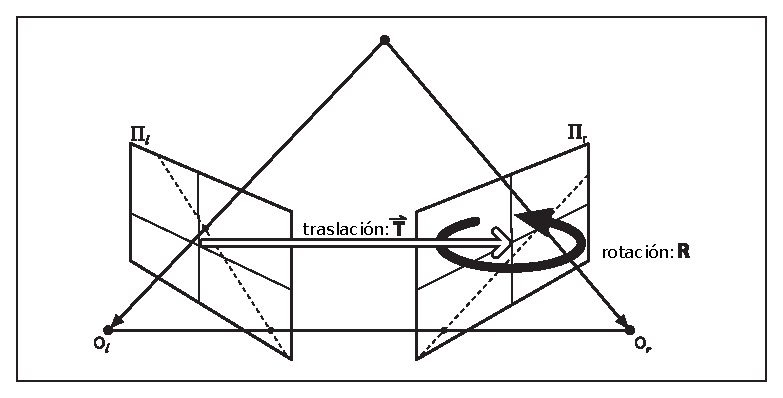
\includegraphics[width=1.0\linewidth]{images/epipolarPlaneRelation}}
        \caption{Rotación y traslación entre dos cámaras}
        \label{fig:epipolarPlaneRelation}
\end{figure}


%*****************************************
%*****************************************
%*****************************************
%*****************************************
%*****************************************
